\begin{Schunk}
\begin{Sinput}
> library("Ham94", lib.loc = "../../../library")
\end{Sinput}
\end{Schunk}
Section 19.2, beginning on page 582 describes cointegration testing of purchasing power parity between
Italian lire and US dollars.  The data used is 100 times log monthly price levels and spot nominal and real
exchange rates, normalized to a value of zero at the start of the series.  
\begin{Schunk}
\begin{Sinput}
> data(ppp, package = "Ham94")
> selection <- subset(ppp, Month >= "1973-01-01" & Month <= "1989-10-01")
> ppp.data <- data.frame(Month = selection$Month, pstar = 100 * 
+     log(selection$PC6IT/selection$PC6IT[[1]]), p = 100 * log(selection$PZUNEW/selection$PZUNEW[[1]]), 
+     ner = -100 * log(selection$EXRITL/selection$EXRITL[[1]]))
> ppp.data[["rer"]] <- ppp.data$p - ppp.data$ner - ppp.data$pstar
\end{Sinput}
\end{Schunk}
\begin{center}
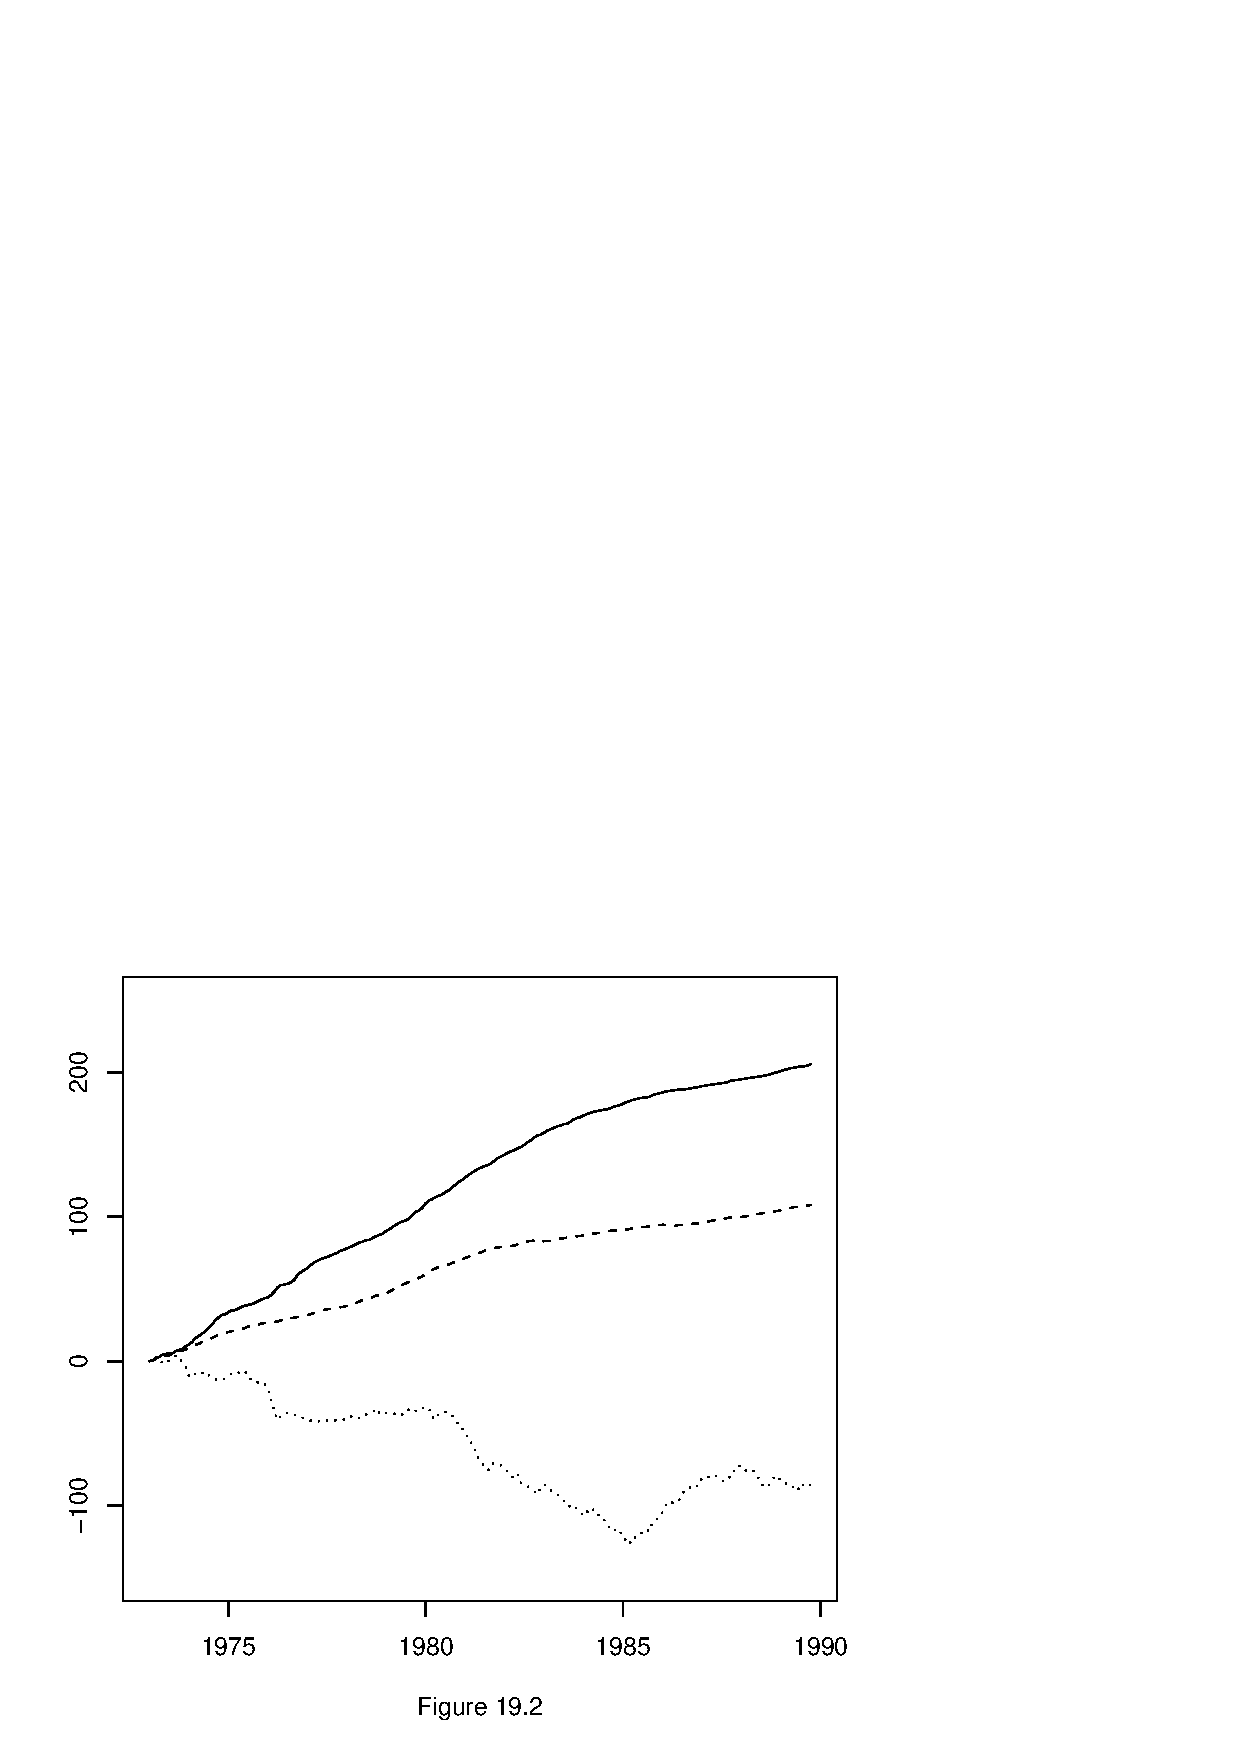
\includegraphics{p582-003}
\end{center}
\begin{center}
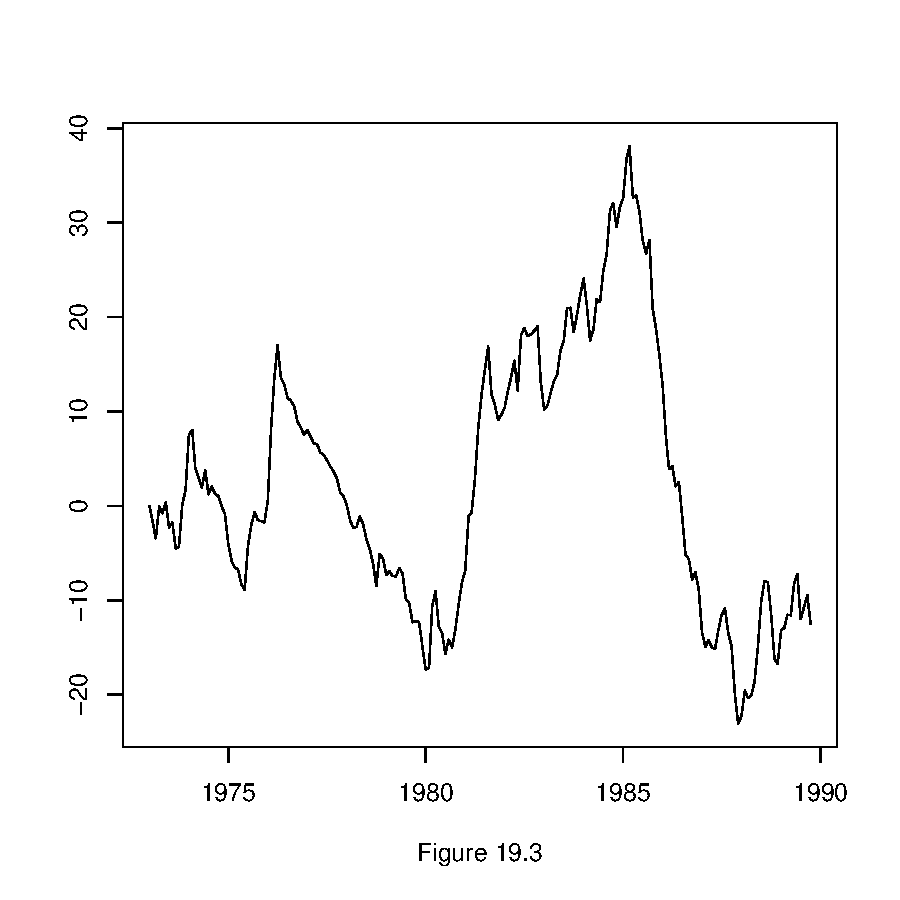
\includegraphics{p582-004}
\end{center}
To save time define a simple utility function to perform augmented Dickey Fuller analysis according to
the conventions in the text.
\begin{Schunk}
\begin{Sinput}
> do.DF <- function(series, lag) {
+     T <- length(series)
+     df.lms <- summary(lm(yt ~ yt_1 + tt + delta.yt_ + 1, list(yt = series[-1:-(lag + 
+         1)], delta.yt_ = embed(diff(series[-T]), lag), yt_1 = series[c(-1:-lag, 
+         -(T:T))], tt = (lag + 2):T)))
+     df.results <- Dickey.Fuller(T = length(series) - lag - 1, 
+         rho = df.lms$coefficients[["yt_1", "Estimate"]], sigma.rho = df.lms$coefficients[["yt_1", 
+             "Std. Error"]], zeta = df.lms$coefficients[paste("delta.yt_", 
+             1:lag, sep = ""), "Estimate"])
+     F <- Wald.F.Test(R = cbind(rep(0, 2), diag(2), rep(0, 2) %o% 
+         rep(0, lag)), b = df.lms$coefficients[, "Estimate"], 
+         r = c(1, 0), s2 = df.lms$sigma^2, XtX_1 = df.lms$cov.unscaled)
+     print(df.lms$coefficients)
+     print(df.results)
+     print(F)
+ }
\end{Sinput}
\end{Schunk}
Following the text, check each series with a Dickey Fuller test with a regression estimated with twelve lags.
\begin{Schunk}
\begin{Sinput}
> for (series.name in c("p", "pstar", "ner", "rer")) do.DF(series = ppp.data[[series.name]], 
+     lag = 12)
\end{Sinput}
\begin{Soutput}
                Estimate  Std. Error     t value      Pr(>|t|)
(Intercept)  0.136160926 0.085779070   1.5873444  1.142502e-01
yt_1         0.994004087 0.003067474 324.0464885 6.323397e-244
tt           0.002927051 0.001766655   1.6568325  9.935541e-02
delta.yt_1   0.553397837 0.075217880   7.3572644  7.109482e-12
delta.yt_2  -0.056908322 0.085440124  -0.6660609  5.062543e-01
delta.yt_3   0.070125117 0.084906900   0.8259060  4.099884e-01
delta.yt_4   0.060389596 0.081969953   0.7367284  4.622797e-01
delta.yt_5  -0.078232496 0.078488461  -0.9967388  3.202754e-01
delta.yt_6  -0.048376861 0.070721885  -0.6840437  4.948576e-01
delta.yt_7   0.165843348 0.068915448   2.4064757  1.715410e-02
delta.yt_8  -0.070207448 0.070014467  -1.0027563  3.173709e-01
delta.yt_9   0.244644550 0.070161410   3.4868819  6.187074e-04
delta.yt_10 -0.110047172 0.072579707  -1.5162251  1.312771e-01
delta.yt_11  0.117580628 0.072937432   1.6120753  1.087579e-01
delta.yt_12  0.046702346 0.068650314   0.6802933  4.972230e-01
$T
[1] 189

$rho
[1] 0.994004

$sigma.rho
[1] 0.003067474

$zeta
 delta.yt_1  delta.yt_2  delta.yt_3  delta.yt_4  delta.yt_5  delta.yt_6 
 0.55339784 -0.05690832  0.07012512  0.06038960 -0.07823250 -0.04837686 
 delta.yt_7  delta.yt_8  delta.yt_9 delta.yt_10 delta.yt_11 delta.yt_12 
 0.16584335 -0.07020745  0.24464455 -0.11004717  0.11758063  0.04670235 

$rho.stat
[1] -10.78352

$t.stat
[1] -1.954675

[1] 2.412933
                Estimate  Std. Error     t value      Pr(>|t|)
(Intercept)  0.768007976 0.253071035   3.0347526  2.776788e-03
yt_1         0.999456707 0.004116999 242.7633949 3.768702e-222
tt          -0.002406065 0.004989081  -0.4822662  6.302229e-01
delta.yt_1   0.420701728 0.076110499   5.5275124  1.170691e-07
delta.yt_2  -0.011592127 0.081521266  -0.1421976  8.870885e-01
delta.yt_3   0.013439685 0.080162382   0.1676558  8.670488e-01
delta.yt_4   0.077206365 0.080125530   0.9635676  3.366000e-01
delta.yt_5  -0.036494296 0.080087139  -0.4556824  6.491866e-01
delta.yt_6   0.145282237 0.078670504   1.8467180  6.648647e-02
delta.yt_7  -0.099118088 0.078839877  -1.2572075  2.103634e-01
delta.yt_8   0.046717520 0.078598766   0.5943798  5.530301e-01
delta.yt_9  -0.049982364 0.078111841  -0.6398820  5.230909e-01
delta.yt_10 -0.034638353 0.078168372  -0.4431249  6.582258e-01
delta.yt_11  0.075555037 0.077993666   0.9687330  3.340230e-01
delta.yt_12  0.021863739 0.073346671   0.2980877  7.659919e-01
$T
[1] 189

$rho
[1] 0.9994567

$sigma.rho
[1] 0.004116999

$zeta
 delta.yt_1  delta.yt_2  delta.yt_3  delta.yt_4  delta.yt_5  delta.yt_6 
 0.42070173 -0.01159213  0.01343968  0.07720637 -0.03649430  0.14528224 
 delta.yt_7  delta.yt_8  delta.yt_9 delta.yt_10 delta.yt_11 delta.yt_12 
-0.09911809  0.04671752 -0.04998236 -0.03463835  0.07555504  0.02186374 

$rho.stat
[1] -0.2382095

$t.stat
[1] -0.1319633

[1] 4.249956
                Estimate  Std. Error     t value      Pr(>|t|)
(Intercept) -0.389337356 0.413800921 -0.94088084  3.480703e-01
yt_1         0.982941298 0.010766440 91.29678192 6.506909e-149
tt          -0.007384125 0.006883901 -1.07266573  2.849066e-01
delta.yt_1   0.348829755 0.074439036  4.68611329  5.595654e-06
delta.yt_2  -0.025567401 0.079110764 -0.32318485  7.469433e-01
delta.yt_3   0.002617322 0.078947706  0.03315261  9.735909e-01
delta.yt_4   0.011689457 0.080007934  0.14610372  8.840086e-01
delta.yt_5   0.099314112 0.079948258  1.24222983  2.158234e-01
delta.yt_6   0.001387289 0.080819939  0.01716518  9.863245e-01
delta.yt_7   0.063205400 0.080614348  0.78404653  4.340788e-01
delta.yt_8   0.117223384 0.080560981  1.45508883  1.474464e-01
delta.yt_9  -0.061127657 0.080788556 -0.75663757  4.502903e-01
delta.yt_10  0.081739596 0.080696462  1.01292665  3.125017e-01
delta.yt_11  0.037261364 0.080646524  0.46203311  6.446347e-01
delta.yt_12 -0.030363466 0.076740775 -0.39566275  6.928385e-01
$T
[1] 189

$rho
[1] 0.9829413

$sigma.rho
[1] 0.01076644

$zeta
  delta.yt_1   delta.yt_2   delta.yt_3   delta.yt_4   delta.yt_5   delta.yt_6 
 0.348829755 -0.025567401  0.002617322  0.011689457  0.099314112  0.001387289 
  delta.yt_7   delta.yt_8   delta.yt_9  delta.yt_10  delta.yt_11  delta.yt_12 
 0.063205400  0.117223384 -0.061127657  0.081739596  0.037261364 -0.030363466 

$rho.stat
[1] -9.112996

$t.stat
[1] -1.584433

[1] 1.489674
                 Estimate  Std. Error     t value      Pr(>|t|)
(Intercept)  0.0532014210 0.390557357  0.13621923  8.918054e-01
yt_1         0.9712932573 0.014145189 68.66597772 5.679805e-128
tt          -0.0004612496 0.003237185 -0.14248477  8.868620e-01
delta.yt_1   0.3178370194 0.074163266  4.28563944  3.010943e-05
delta.yt_2  -0.0149166870 0.078078854 -0.19104644  8.487119e-01
delta.yt_3   0.0127973250 0.077727723  0.16464299  8.694161e-01
delta.yt_4   0.0224258044 0.078676900  0.28503671  7.759550e-01
delta.yt_5   0.0845155831 0.078339518  1.07883716  2.821536e-01
delta.yt_6  -0.0030653274 0.079071534 -0.03876651  9.691210e-01
delta.yt_7   0.0299137752 0.078750797  0.37985362  7.045173e-01
delta.yt_8   0.0824197050 0.078641636  1.04804158  2.960730e-01
delta.yt_9  -0.0478615036 0.078647910 -0.60855405  5.436137e-01
delta.yt_10  0.0755667133 0.078405880  0.96378886  3.364893e-01
delta.yt_11  0.0504082264 0.078279945  0.64394816  5.204570e-01
delta.yt_12 -0.0124704308 0.075997755 -0.16408946  8.698512e-01
$T
[1] 189

$rho
[1] 0.9712933

$sigma.rho
[1] 0.01414519

$zeta
  delta.yt_1   delta.yt_2   delta.yt_3   delta.yt_4   delta.yt_5   delta.yt_6 
 0.317837019 -0.014916687  0.012797325  0.022425804  0.084515583 -0.003065327 
  delta.yt_7   delta.yt_8   delta.yt_9  delta.yt_10  delta.yt_11  delta.yt_12 
 0.029913775  0.082419705 -0.047861504  0.075566713  0.050408226 -0.012470431 

$rho.stat
[1] -13.48204

$t.stat
[1] -2.029435

[1] 2.078078
\end{Soutput}
\end{Schunk}
Now check the real exchange rate with a Phillips Perron test

\begin{Schunk}
\begin{Sinput}
> pp.lms <- summary(lm(zt ~ zt_1 + 1, data.frame(zt = ppp.data$rer[-1], 
+     zt_1 = ppp.data$rer[-length(ppp.data$rer)])))
> PP.results <- Phillips.Perron(T = length(pp.lms$residuals), rho = pp.lms$coefficients[["zt_1", 
+     "Estimate"]], sigma.rho = pp.lms$coefficients[["zt_1", "Std. Error"]], 
+     s = pp.lms$sigma, lambda.hat.sq = as.numeric(Newey.West(pp.lms$residuals %o% 
+         1, 12)), gamma0 = mean(pp.lms$residuals^2))
> print(pp.lms$coefficients)
\end{Sinput}
\begin{Soutput}
              Estimate Std. Error    t value      Pr(>|t|)
(Intercept) -0.0297931 0.17835718 -0.1670418  8.675068e-01
zt_1         0.9865420 0.01275287 77.3584248 1.854719e-150
\end{Soutput}
\begin{Sinput}
> print(PP.results)
\end{Sinput}
\begin{Soutput}
$T
[1] 201

$rho
[1] 0.986542

$sigma.rho
[1] 0.01275287

$s.sq
[1] 6.205887

$lambda.hat.sq
[1] 13.03064

$gamma0
[1] 6.144137

$rho.stat
[1] -6.35068

$t.stat
[1] -1.706128
\end{Soutput}
\end{Schunk}

Estimating the impulse response function gives a sense of the persistence of deviations from PPP.
\begin{Schunk}
\begin{Sinput}
> ar.results <- ar(ppp.data$rer, aic = FALSE, order.max = 13, method = "ols", 
+     demean = TRUE)
> tt <- seq(1, 72)
> start.innov <- rep(0, 13)
> et <- c(start.innov, 1, rep(0, length(tt) - 14))
> arima.sim.output <- arima.sim(list(order = c(13, 0, 0), ar = ar.results$ar), 
+     n = length(tt), innov = et, n.start = length(start.innov), 
+     start.innov = start.innov)
> irf <- as.vector(arima.sim.output)
\end{Sinput}
\end{Schunk}
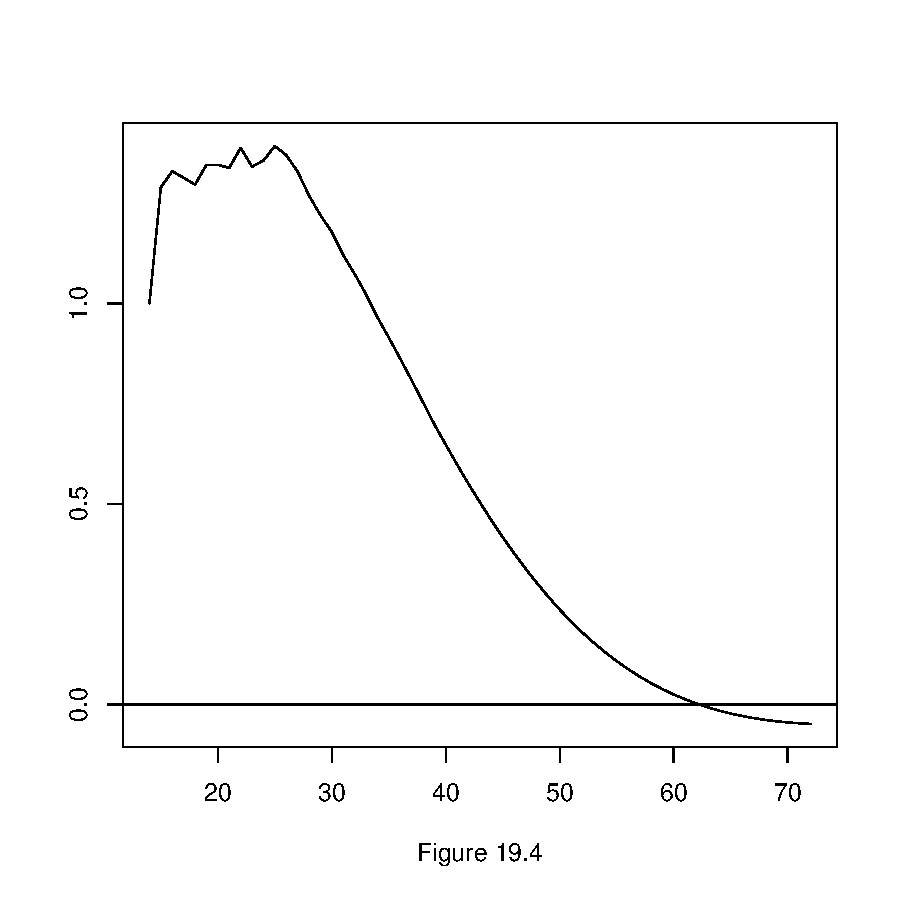
\includegraphics{p582-009}
\subsection{Estimating the Cointegrating Vector}
Page 598 shows an example of the Phillips Ouliaris Hansen procedure for estimating a cointegrating vector.
\begin{Schunk}
\begin{Sinput}
> poh.cointegration.lm <- lm(p ~ 1 + ner + pstar, ppp.data)
> poh.residual.lms <- summary(lm(u ~ 0 + u_1, data.frame(u = poh.cointegration.lm$residuals[-1], 
+     u_1 = poh.cointegration.lm$residuals[-length(poh.cointegration.lm$residuals)])))
> POH.results <- Phillips.Perron(T = length(poh.residual.lms$residuals), 
+     rho = poh.residual.lms$coefficients[["u_1", "Estimate"]], 
+     sigma.rho = poh.residual.lms$coefficients[["u_1", "Std. Error"]], 
+     s = poh.residual.lms$sigma, lambda.hat.sq = as.numeric(Newey.West(poh.residual.lms$residuals %o% 
+         1, 12)), gamma0 = mean(poh.residual.lms$residuals^2))
> print(summary(poh.cointegration.lm)$coefficients)
\end{Sinput}
\begin{Soutput}
              Estimate  Std. Error   t value      Pr(>|t|)
(Intercept) 2.71231296 0.367695493  7.376519  4.298888e-12
ner         0.05134848 0.012045369  4.262923  3.114337e-05
pstar       0.53004097 0.006708385 79.011705 3.148050e-152
\end{Soutput}
\begin{Sinput}
> print(poh.residual.lms$coefficients)
\end{Sinput}
\begin{Soutput}
     Estimate Std. Error  t value     Pr(>|t|)
u_1 0.9833108 0.01171956 83.90338 7.71577e-158
\end{Soutput}
\begin{Sinput}
> print(POH.results)
\end{Sinput}
\begin{Soutput}
$T
[1] 201

$rho
[1] 0.9833108

$sigma.rho
[1] 0.01171956

$s.sq
[1] 0.1630028

$lambda.hat.sq
[1] 0.4082242

$gamma0
[1] 0.1621919

$rho.stat
[1] -7.542281

$t.stat
[1] -2.020981
\end{Soutput}
\end{Schunk}
A second example performs a similar analysis on quarterly US consumption and income data from 1947Q1 to 1989Q4.
\begin{Schunk}
\begin{Sinput}
> data(coninc, package = "Ham94")
> selection <- subset(coninc, Quarter >= "1947-01-01" & Quarter <= 
+     "1989-07-01")
> coninc.data <- data.frame(Quarter = selection$Quarter, cons = 100 * 
+     log(selection$GC82), inc = 100 * log(selection$GYD82))
\end{Sinput}
\end{Schunk}
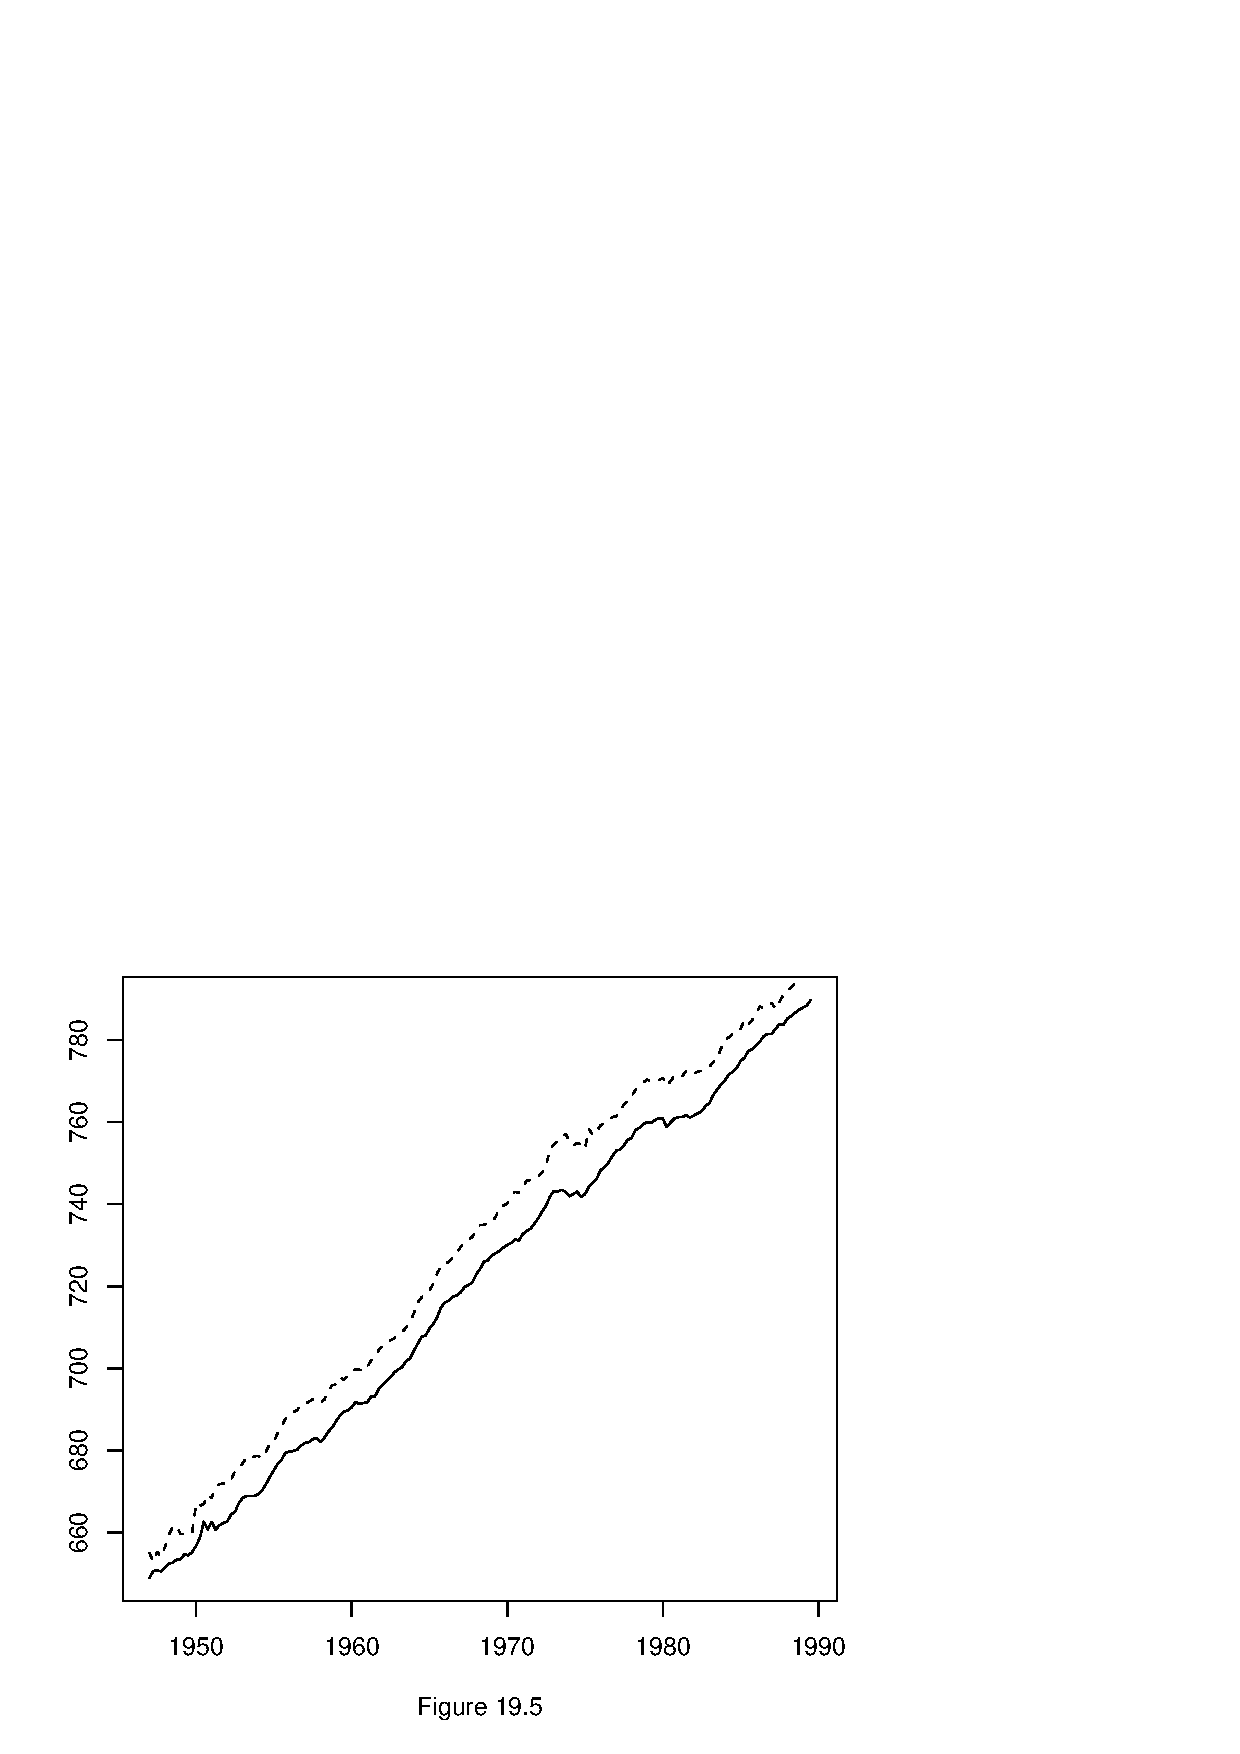
\includegraphics{p582-012}
Test individual series for unit root status using Dickey Fuller.
\begin{Schunk}
\begin{Sinput}
> for (series.name in c("inc", "cons")) do.DF(series = coninc.data[[series.name]], 
+     lag = 6)
\end{Sinput}
\begin{Soutput}
                Estimate  Std. Error     t value     Pr(>|t|)
(Intercept) 20.336729221 15.04162460  1.35203010 1.783352e-01
yt_1         0.970584904  0.02306293 42.08419931 1.029200e-86
tt           0.023796844  0.01985318  1.19864142 2.324968e-01
delta.yt_1  -0.006528755  0.08092856 -0.08067307 9.358060e-01
delta.yt_2  -0.035846316  0.08025935 -0.44663103 6.557649e-01
delta.yt_3   0.102128545  0.07758036  1.31642276 1.899755e-01
delta.yt_4  -0.187536343  0.07699406 -2.43572477 1.599577e-02
delta.yt_5  -0.037187883  0.07813842 -0.47592314 6.347992e-01
delta.yt_6   0.027855951  0.07662877  0.36351818 7.167132e-01
$T
[1] 164

$rho
[1] 0.970585

$sigma.rho
[1] 0.02306293

$zeta
  delta.yt_1   delta.yt_2   delta.yt_3   delta.yt_4   delta.yt_5   delta.yt_6 
-0.006528755 -0.035846316  0.102128545 -0.187536343 -0.037187883  0.027855951 

$rho.stat
[1] -4.242382

$t.stat
[1] -1.275428

[1] 1.132134
               Estimate  Std. Error    t value     Pr(>|t|)
(Intercept) 29.46860131 15.19248322  1.9396830 5.423391e-02
yt_1         0.95552168  0.02360001 40.4881863 2.508405e-84
tt           0.03721088  0.02006161  1.8548306 6.552012e-02
delta.yt_1   0.03624864  0.07979877  0.4542506 6.502840e-01
delta.yt_2   0.25964745  0.07935028  3.2721680 1.315743e-03
delta.yt_3   0.06273192  0.08172798  0.7675697 4.439106e-01
delta.yt_4  -0.05234112  0.08122252 -0.6444163 5.202580e-01
delta.yt_5  -0.04791625  0.07956524 -0.6022260 5.479037e-01
delta.yt_6  -0.06782142  0.07919698 -0.8563637 3.931186e-01
$T
[1] 164

$rho
[1] 0.9555217

$sigma.rho
[1] 0.02360001

$zeta
 delta.yt_1  delta.yt_2  delta.yt_3  delta.yt_4  delta.yt_5  delta.yt_6 
 0.03624864  0.25964745  0.06273192 -0.05234112 -0.04791625 -0.06782142 

$rho.stat
[1] -9.011597

$t.stat
[1] -1.884673

[1] 1.858290
\end{Soutput}
\end{Schunk}
Estimate cointegration vector, then check for unit root status of the residual using Phillips Perron.
\begin{Schunk}
\begin{Sinput}
> poh.cointegration.lm <- lm(cons ~ 1 + inc, coninc.data)
> poh.residual.lms <- summary(lm(u ~ 0 + u_1, data.frame(u = poh.cointegration.lm$residuals[-1], 
+     u_1 = poh.cointegration.lm$residuals[-length(poh.cointegration.lm$residuals)])))
> POH.results <- Phillips.Perron(T = length(poh.residual.lms$residuals), 
+     rho = poh.residual.lms$coefficients[["u_1", "Estimate"]], 
+     sigma.rho = poh.residual.lms$coefficients[["u_1", "Std. Error"]], 
+     s = poh.residual.lms$sigma, lambda.hat.sq = as.numeric(Newey.West(poh.residual.lms$residuals %o% 
+         1, 6)), gamma0 = mean(poh.residual.lms$residuals^2))
> print(summary(poh.cointegration.lm)$coefficients)
\end{Sinput}
\begin{Soutput}
             Estimate  Std. Error     t value      Pr(>|t|)
(Intercept) 0.6675807 2.350348907   0.2840347  7.767315e-01
inc         0.9864943 0.003217444 306.6080542 5.567137e-234
\end{Soutput}
\begin{Sinput}
> print(poh.residual.lms$coefficients)
\end{Sinput}
\begin{Soutput}
     Estimate Std. Error  t value     Pr(>|t|)
u_1 0.7818542 0.04788553 16.32757 1.402076e-36
\end{Soutput}
\begin{Sinput}
> print(POH.results)
\end{Sinput}
\begin{Soutput}
$T
[1] 170

$rho
[1] 0.7818542

$sigma.rho
[1] 0.04788553

$s.sq
[1] 1.22395

$lambda.hat.sq
[1] 1.030594

$gamma0
[1] 1.216750

$rho.stat
[1] -32.04525

$t.stat
[1] -4.27529
\end{Soutput}
\end{Schunk}
\subsection{Testing Hypotheses About the Cointegrating Vector}
Page 608-612 illustrate a technique that uses leads and lags to produce a stationary
vector for hypothesis testing.
\begin{Schunk}
\begin{Sinput}
> T <- length(coninc.data$Quarter)
> lead.lag.data <- list(ct = coninc.data$cons[c(-1:-5, -((T - 3):T))], 
+     yt = coninc.data$inc[c(-1:-5, -((T - 3):T))], delta.yt = diff(coninc.data$inc[c(-1:-4, 
+         -((T - 3):T))]), delta.yt_ = embed(diff(coninc.data$inc[-((T - 
+         4):T)]), 4), delta.yt. = embed(diff(coninc.data$inc[-1:-5])[(T - 
+         6):1], 4)[(T - 9):1, ], tt = 6:(T - 4))
\end{Sinput}
\end{Schunk}
The regression is estimated with both no trend and trend, and the corrected t-stat is calculated.
\begin{Schunk}
\begin{Sinput}
> no.trend.lm <- lm(ct ~ 1 + yt + delta.yt. + delta.yt + delta.yt_, 
+     lead.lag.data)
> trend.lm <- lm(ct ~ 1 + yt + tt + delta.yt. + delta.yt + delta.yt_, 
+     lead.lag.data)
> for (model in list(no.trend.lm, trend.lm)) {
+     lags <- 2
+     cms <- summary(model)
+     T <- length(cms$residuals)
+     cfs <- cms$coefficients
+     t.rho <- (cfs[["yt", "Estimate"]] - 1)/cfs[["yt", "Std. Error"]]
+     rms <- summary(lm(u ~ 0 + u_, list(u = cms$residuals[-c(1:lags)], 
+         u_ = embed(cms$residuals[-T], lags))))
+     sigma1.hat.sq <- mean(rms$residuals^2)
+     lambda.11 <- sigma1.hat.sq^0.5/(1 - sum(rms$coefficients[paste("u_", 
+         1:lags, sep = ""), "Estimate"]))
+     t.a <- t.rho * cms$sigma/lambda.11
+     print(cfs)
+     print(rms$coefficients)
+     print(T)
+     print(cms$sigma)
+     print(t.rho)
+     print(sigma1.hat.sq)
+     print(lambda.11)
+     print(t.a)
+ }
\end{Sinput}
\begin{Soutput}
               Estimate  Std. Error     t value      Pr(>|t|)
(Intercept) -4.51922906 2.340224673  -1.9311091  5.534290e-02
yt           0.99215853 0.003063317 323.8837231 1.617626e-216
delta.yt.1   0.48592391 0.115704789   4.1996871  4.551158e-05
delta.yt.2   0.26411856 0.114892015   2.2988418  2.288546e-02
delta.yt.3   0.28614193 0.115594505   2.4753939  1.441397e-02
delta.yt.4   0.14530952 0.118799555   1.2231487  2.231790e-01
delta.yt    -0.24036007 0.117415901  -2.0470828  4.238356e-02
delta.yt_1  -0.01101143 0.113899420  -0.0966768  9.231113e-01
delta.yt_2   0.06969114 0.111505773   0.6250003  5.329142e-01
delta.yt_3   0.04055551 0.111155199   0.3648548  7.157303e-01
delta.yt_4   0.02150153 0.110083985   0.1953193  8.454056e-01
     Estimate Std. Error  t value     Pr(>|t|)
u_1 0.7179687 0.07722647 9.296924 1.127578e-16
u_2 0.2057401 0.07684783 2.677241 8.207043e-03
[1] 162
[1] 1.516006
[1] -2.559799
[1] 0.3809180
[1] 8.089864
[1] -0.4796954
                Estimate  Std. Error    t value     Pr(>|t|)
(Intercept) 198.87166510 15.01478288 13.2450577 5.215628e-27
yt            0.68117915  0.02292367 29.7150967 9.919458e-65
tt            0.26895671  0.01974617 13.6207037 5.213974e-28
delta.yt.1    0.40061828  0.07787309  5.1445023 8.270282e-07
delta.yt.2    0.15407283  0.07749787  1.9880910 4.862147e-02
delta.yt.3    0.16559666  0.07805023  2.1216678 3.550904e-02
delta.yt.4    0.02782397  0.08016237  0.3470952 7.290063e-01
delta.yt     -0.05124600  0.07998305 -0.6407108 5.226882e-01
delta.yt_1    0.12737594  0.07708222  1.6524685 1.005308e-01
delta.yt_2    0.23116996  0.07573754  3.0522506 2.687346e-03
delta.yt_3    0.20472613  0.07553655  2.7102923 7.505953e-03
delta.yt_4    0.18997478  0.07487875  2.5370986 1.219919e-02
     Estimate Std. Error  t value     Pr(>|t|)
u_1 0.6871713 0.07786238 8.825460 1.937474e-15
u_2 0.1291820 0.07666487 1.685022 9.395837e-02
[1] 162
[1] 1.017016
[1] -13.90793
[1] 0.3439489
[1] 3.193478
[1] -4.429212
\end{Soutput}
\end{Schunk}

